\documentclass[11pt,a4paper]{article}

% ====================================================================
% Packages
% ====================================================================
\usepackage[utf8]{inputenc}
\usepackage[T1]{fontenc}
\usepackage{amsmath,amssymb,amsthm}
\usepackage{mathtools}
\usepackage{hyperref}
\usepackage[margin=1in]{geometry}
\usepackage{enumitem}
\usepackage{booktabs}
\usepackage{listings}
\usepackage{xcolor}
\usepackage{cleveref}
\usepackage[numbers]{natbib}
\usepackage{mdframed}
\usepackage{tikz}
\usetikzlibrary{arrows.meta,positioning,decorations.pathreplacing}

% ====================================================================
% Theorem environments
% ====================================================================
\theoremstyle{plain}
\newtheorem{theorem}{Theorem}[section]
\newtheorem{lemma}[theorem]{Lemma}
\newtheorem{proposition}[theorem]{Proposition}
\newtheorem{corollary}[theorem]{Corollary}

\theoremstyle{definition}
\newtheorem{definition}[theorem]{Definition}
\newtheorem{remark}[theorem]{Remark}

% ====================================================================
% Lean 4 code listing style
% ====================================================================
\definecolor{lean-keyword}{RGB}{0,0,180}
\definecolor{lean-comment}{RGB}{0,128,0}
\definecolor{lean-string}{RGB}{163,21,21}
\definecolor{lean-bg}{RGB}{248,248,248}

\lstdefinelanguage{lean4}{
  keywords={theorem,lemma,def,class,instance,import,open,variable,
            noncomputable,section,namespace,end,where,let,have,show,
            intro,obtain,use,exact,rw,simp,apply,by,fun,match,if,
            then,else,do,return,axiom,abbrev,private,attribute,
            suffices,change,congr,ext,constructor,rintro,push_neg,
            linarith,absurd,set_option,omit,in,set,cases,refine,
            calc,filter_upwards,with,specialize,unfold,structure},
  sensitive=true,
  morecomment=[l]{--},
  morecomment=[n]{/-}{-/},
  morestring=[b]",
  literate=
    {\\to}{$\to$}1
    {\\lam}{$\lambda$}1
    {\\forall}{$\forall$}1
    {\\exists}{$\exists$}1
    {\\le}{$\le$}1
    {\\ge}{$\ge$}1
    {\\ne}{$\ne$}1
    {\\and}{$\wedge$}1
    {\\or}{$\vee$}1
    {\\not}{$\neg$}1
    {\\iff}{$\leftrightarrow$}1
    {\\mapsto}{$\mapsto$}1
    {\\sub}{$\subset$}1
}

\lstset{
  language=lean4,
  basicstyle=\small\ttfamily,
  keywordstyle=\color{lean-keyword}\bfseries,
  commentstyle=\color{lean-comment}\itshape,
  stringstyle=\color{lean-string},
  backgroundcolor=\color{lean-bg},
  frame=single,
  framerule=0.5pt,
  breaklines=true,
  breakatwhitespace=true,
  tabsize=2,
  showstringspaces=false,
  numbers=none,
  xleftmargin=2em,
  framexleftmargin=1.5em,
  columns=flexible,
}

% ====================================================================
% Custom commands
% ====================================================================
\newcommand{\LLPO}{\mathsf{LLPO}}
\newcommand{\WLPO}{\mathsf{WLPO}}
\newcommand{\LPO}{\mathsf{LPO}}
\newcommand{\BISH}{\mathsf{BISH}}
\newcommand{\IVT}{\mathsf{IVT}}
\newcommand{\ExactIVT}{\mathsf{ExactIVT}}
\newcommand{\ApproxIVT}{\mathsf{ApproxIVT}}
\newcommand{\CHSH}{\mathsf{CHSH}}
\newcommand{\lean}[1]{\lstinline[language=lean4]{#1}}

% ====================================================================
% Title
% ====================================================================
\title{The Logical Cost of Root-Finding:\\
LLPO, the Intermediate Value Theorem,\\
and Bell Angle Optimization\\[6pt]
\large A Lean~4 Formalization}

\author{Foundation--Relativity Project, Paper~27}
\date{\today}

% ====================================================================
\begin{document}
\maketitle

\begin{abstract}
We formalize in Lean~4 the equivalence between the Lesser Limited Principle
of Omniscience ($\LLPO$) and the exact Intermediate Value Theorem ($\ExactIVT$),
and show that Bell angle optimization for general quantum states reduces to
IVT instances.  The main results are:
(i)~$\LLPO \leftrightarrow \ExactIVT$ (axiomatized from Bridges--Richman 1987);
(ii)~finding measurement angles that witness a CHSH violation above the classical
bound~2 is an IVT problem, hence requires~$\LLPO$;
(iii)~a three-level stratification placing Bell angle-finding strictly below
gap detection ($\WLPO$, Paper~26) in the constructive hierarchy.
The formalization compiles with zero \texttt{sorry} statements and six
axioms, all with published citations.
This paper extends Paper~21's abstract $\LLPO \leftrightarrow
\mathsf{BellSignDecision}$ result by identifying the \emph{mechanism}:
the Intermediate Value Theorem is why $\LLPO$ appears in Bell physics.
\end{abstract}

% ====================================================================
\section{Introduction}\label{sec:intro}
% ====================================================================

\subsection{Context and Motivation}

Paper~21 of this series established that $\LLPO$ is equivalent to a
Bell sign-decision principle: for binary sequences with at most one~1,
determining whether the~1 sits at an even or odd index is equivalent to
the capacity to resolve sign ambiguities in Bell asymmetry
parameters~\cite{P21}.  That result was algebraic---it encoded binary
sequences into geometric-series sums and read off sign decisions.
The equivalence was proved but the \emph{reason} LLPO appears in
Bell physics remained unexplained.

This paper identifies the mechanism.  The Intermediate Value Theorem
(IVT)---the assertion that a continuous function with a sign change on
a closed interval has a root---is equivalent to $\LLPO$ over Bishop-style
constructive mathematics ($\BISH$).  This equivalence was established by
Bridges and Richman~\cite{BridgesRichman1987} and
Ishihara~\cite{Ishihara1989}.  Bell angle optimization, the problem of
finding measurement angles that maximize the CHSH violation for a general
quantum state, reduces to root-finding for continuous functions of the
measurement angles.  Therefore, Bell angle-finding costs exactly~$\LLPO$.

\subsection{The Constructive Hierarchy}

The hierarchy of omniscience principles over $\BISH$ provides a
fine-grained complexity classification for problems in analysis and
physics:
\[
  \BISH \;\subsetneq\; \LLPO \;\subsetneq\; \WLPO \;\subsetneq\; \LPO.
\]
Each level adds a specific decision capability:
\begin{itemize}[nosep]
  \item $\LPO$: for any binary sequence, either all entries are~0 or
    some entry is~1.
  \item $\WLPO$: for any binary sequence, either all entries are~0 or it
    is not the case that all are~0.
  \item $\LLPO$: for a binary sequence with at most one~1, either all
    even-indexed entries are~0 or all odd-indexed are~0.
\end{itemize}
Paper~26 showed that gap detection in the bidual quotient $\ell^\infty/c_0$
calibrates at~$\WLPO$.  This paper shows that Bell angle-finding
calibrates one level lower, at~$\LLPO$.

\subsection{Contributions}

\begin{enumerate}[nosep]
  \item A Lean~4 formalization of $\LLPO \leftrightarrow \ExactIVT$
    (axiomatized from the published literature).
  \item A reduction of Bell angle optimization to IVT instances:
    the single-angle CHSH slice is a continuous function whose threshold
    crossings are IVT problems.
  \item A three-level stratification theorem:
    \begin{itemize}[nosep]
      \item Level~1 ($\BISH$): CHSH bound and specific-angle violation
        are computable.
      \item Level~2 ($\LLPO$): finding general optimal angles requires IVT.
      \item Level~3 (hierarchy): $\WLPO \to \LLPO$ strictly, so
        angle-finding is strictly easier than gap detection.
    \end{itemize}
  \item Zero \texttt{sorry} statements; six axioms with published citations.
\end{enumerate}

\subsection{Scope and Limitations}

This paper establishes a \emph{forward-direction calibration}: $\LLPO$
suffices for Bell angle-finding via IVT, and angle-finding produces IVT
instances.  We do \emph{not} prove a full correspondence (encoding
arbitrary IVT instances into quantum correlations), which would require
constructing quantum states from continuous functions---a substantially
harder problem.  Paper~26's experience demonstrated that engineering
embeddings into abstract spaces can produce technically correct but
conceptually inflated results.  We keep the present work grounded:
$\LLPO \leftrightarrow \IVT$ is established mathematics; angle-finding as
IVT application is established physics; together they explain Paper~21's
result rather than restating it.

% ====================================================================
\section{Omniscience Principles}\label{sec:omniscience}
% ====================================================================

\begin{definition}[AtMostOne]\label{def:atmostone}
A binary sequence $\alpha : \mathbb{N} \to \{0,1\}$ has \emph{at most
one}~1 if $\alpha(m) = 1$ and $\alpha(n) = 1$ imply $m = n$.
\end{definition}

\begin{definition}[$\LLPO$]\label{def:llpo}
For every binary sequence $\alpha$ with at most one~1, either all
even-indexed entries are~0, or all odd-indexed entries are~0:
\[
  \forall \alpha.\;
    \mathrm{AtMostOne}(\alpha) \;\Longrightarrow\;
    (\forall n.\; \alpha(2n) = 0)
    \;\lor\;
    (\forall n.\; \alpha(2n+1) = 0).
\]
\end{definition}

The hierarchy $\LPO \to \WLPO \to \LLPO$ is proved in
\texttt{Basic.lean} (lines~65--94).  All implications are strict over
$\BISH$~\cite{BridgesRichman1987}.

\begin{lstlisting}
theorem lpo_implies_wlpo : LPO -> WLPO
theorem wlpo_implies_llpo : WLPO -> LLPO
theorem lpo_implies_llpo : LPO -> LLPO
\end{lstlisting}

% ====================================================================
\section{The Intermediate Value Theorem}\label{sec:ivt}
% ====================================================================

\begin{definition}[$\ExactIVT$]\label{def:exactivt}
If $f : \mathbb{R} \to \mathbb{R}$ is continuous with $f(0) < 0$ and
$f(1) > 0$, then there exists $x \in [0,1]$ with $f(x) = 0$.
\end{definition}

\begin{definition}[$\ApproxIVT$]\label{def:approxivt}
Under the same hypotheses, for every $\varepsilon > 0$ there exists
$x \in [0,1]$ with $|f(x)| < \varepsilon$.
\end{definition}

The approximate IVT is $\BISH$-valid: bisection converges to an
approximate root without requiring sign decisions at each
step~\cite{BishopBridges1985}.  The exact IVT requires resolving whether
$f(\text{midpoint}) \le 0$ or $f(\text{midpoint}) \ge 0$ at each
bisection step, which is precisely the real-number sign decision that
$\LLPO$ provides.

\begin{theorem}[Bridges--Richman 1987, Ishihara 1989]\label{thm:ivt-llpo}
$\ExactIVT \leftrightarrow \LLPO$ over $\BISH$.
\end{theorem}

This equivalence is axiomatized in our formalization:

\begin{lstlisting}
axiom exact_ivt_iff_llpo : ExactIVT <-> LLPO
\end{lstlisting}

The forward direction ($\ExactIVT \to \LLPO$) constructs a continuous
piecewise-linear function from a binary sequence with at most one~1,
whose root position encodes the even/odd
decision~\cite{BridgesRichman1987}.
The backward direction ($\LLPO \to \ExactIVT$) uses $\LLPO$ to resolve
sign ambiguities in bisection, via the real sign decision principle
$\LLPO \to \forall x : \mathbb{R}.\; x \le 0 \lor 0 \le x$
\cite{Ishihara2006}.

We prove several derived results: $\ExactIVT$ implies $\ApproxIVT$
(trivially), and $\ExactIVT$ on $[0,1]$ implies the generalized IVT on
arbitrary $[a,b]$ by affine rescaling (\texttt{IVT.lean}, lines~102--148).

% ====================================================================
\section{Continuous Bell Correlations}\label{sec:bell}
% ====================================================================

\subsection{The Correlation Framework}

We model Bell correlations as continuous functions of measurement angles,
rather than using the matrix formalism of Paper~11.  This is natural for
the IVT connection: the CHSH value is a continuous function of angles,
and finding optimal angles is a root-finding problem.

\begin{definition}[BellCorrelation]\label{def:bellcorrelation}
A \emph{Bell correlation} is a function $E : \mathbb{R} \times
\mathbb{R} \to \mathbb{R}$ that is:
\begin{enumerate}[nosep]
  \item continuous in both angles (jointly), and
  \item bounded: $|E(\theta_1, \theta_2)| \le 1$ for all $\theta_1, \theta_2$.
\end{enumerate}
\end{definition}

\begin{lstlisting}
structure BellCorrelation where
  E : R -> R -> R
  E_continuous : Continuous (fun p : R * R => E p.1 p.2)
  E_bound : forall t1 t2, |E t1 t2| <= 1
\end{lstlisting}

\begin{definition}[CHSH value]\label{def:chsh}
For a Bell correlation $B$ and four measurement angles
$a, a', b, b'$:
\[
  S(a, a', b, b') \;=\;
    E(a,b) + E(a,b') + E(a',b) - E(a',b').
\]
\end{definition}

\subsection{The Singlet State}

The canonical example is the Bell singlet state $|\psi^-\rangle$, whose
correlation function is $E(\theta_A, \theta_B) = -\cos(\theta_A -
\theta_B)$.  We prove continuity and boundedness, assembling the
singlet as a \lean{BellCorrelation} instance (\texttt{BellCorrelation.lean},
lines~81--102).

\subsection{Classical Bound and Quantum Violation}

The classical CHSH bound $|S| \le 2$ for local hidden variable (LHV)
models is axiomatized in the measure-theoretic formulation.  The quantum
violation $|S| > 2$ for the singlet state at the Tsirelson angles is
also axiomatized (the trigonometric computation $S = 2\sqrt{2}$ was
proved in Paper~11 in matrix form).

We prove $S_{\text{quantum}} = 2\sqrt{2} > 2$ directly:

\begin{lstlisting}
theorem S_quantum_gt_two : S_quantum > 2
\end{lstlisting}

\subsection{The CHSH Slice}

The key construction for the IVT connection is the \emph{CHSH slice}:
fixing three angles $a', b, b'$ and letting the fourth angle $a$ vary:

\begin{definition}[CHSH slice]\label{def:chshslice}
$\text{chshSlice}(B, a', b, b')(a) = S(a, a', b, b')$.
\end{definition}

This is a continuous function of one real variable
(\texttt{BellCorrelation.lean}, lines~67--84).  The reduction from~4D
optimization to~1D root-finding passes through this construction.

% ====================================================================
\section{Angle-Finding as an IVT Instance}\label{sec:angle}
% ====================================================================

\subsection{IVT Instances}

\begin{definition}[IVT instance]\label{def:ivtinstance}
An \emph{IVT instance} consists of:
\begin{itemize}[nosep]
  \item an interval $[a,b]$ with $a < b$,
  \item a continuous function $f : \mathbb{R} \to \mathbb{R}$,
  \item $f(a) < 0$ and $f(b) > 0$ (sign change).
\end{itemize}
\end{definition}

Every IVT instance has a root given $\LLPO$:

\begin{lstlisting}
theorem ivt_instance_has_root (hllpo : LLPO) (I : IVTInstance) :
    I.hasRoot
\end{lstlisting}

\subsection{Threshold Crossings}

Finding where a continuous function $g$ crosses a threshold $c$ reduces
to root-finding: set $f(x) = g(x) - c$ and apply IVT.

\begin{lstlisting}
def thresholdCrossing (g : R -> R) (hcont : Continuous g)
    (a b c : R) (hab : a < b) (hga : g a < c) (hgb : c < g b) :
    IVTInstance
\end{lstlisting}

\subsection{The Core Reduction}

The core reduction is:

\begin{theorem}\label{thm:single-angle-ivt}
If the CHSH slice for a Bell correlation $B$ (with three angles fixed)
takes values both below and above a threshold~$c$ at angles $\theta_1 <
\theta_2$, then finding the crossing point is an IVT instance.
Given $\LLPO$, the crossing angle exists.
\end{theorem}

\begin{lstlisting}
theorem single_angle_ivt (B : BellCorrelation) (a' b b' : R)
    (c : R) (t1 t2 : R) (h12 : t1 < t2)
    (h_below : chshSlice B a' b b' t1 < c)
    (h_above : c < chshSlice B a' b b' t2)
    (hllpo : LLPO) :
    exists a, t1 <= a /\ a <= t2 /\ chshSlice B a' b b' a = c
\end{lstlisting}

For a Bell correlation with a CHSH violation $|S| > 2$, the axiom
\lean{chsh_slice_sign_change} asserts that there exist fixed angles
$a', b, b'$ and an interval $[\theta_1, \theta_2]$ on which the CHSH
slice crosses the classical threshold~2.  This is a physical fact: as
the measurement angle varies continuously, the CHSH value interpolates
between classical ($|S| \le 2$) and maximally nonlocal
($|S| = 2\sqrt{2}$) regimes.

\begin{theorem}\label{thm:llpo-crossing}
Given $\LLPO$ and a Bell correlation with $|S| > 2$, there exist angles
$a'_0, b_0, b'_0, a_0$ such that $\text{chshSlice}(B, a'_0, b_0,
b'_0)(a_0) = 2$.
\end{theorem}

\begin{lstlisting}
theorem llpo_finds_crossing (hllpo : LLPO) (B : BellCorrelation)
    (hviol : exists a a' b b', |chshValue B a a' b b'| > 2) :
    exists a0 b0 b0' a0, chshSlice B a0 b0 b0' a0 = 2
\end{lstlisting}

% ====================================================================
\section{Calibration}\label{sec:calibration}
% ====================================================================

\subsection{The Central Equivalence}

The foundation of the paper is the known equivalence:

\begin{theorem}\label{thm:llpo-ivt}
$\LLPO \leftrightarrow \ExactIVT$.
\end{theorem}

\begin{lstlisting}
theorem llpo_iff_exactIVT : LLPO <-> ExactIVT
\end{lstlisting}

\subsection{The Calibration Chain}

The calibration chain connects the omniscience hierarchy to Bell
angle-finding:
\[
  \LLPO \;\xleftrightarrow{\text{Bridges--Richman}}\;
  \ExactIVT \;\xrightarrow{\text{threshold crossing}}\;
  \text{angle crossings findable}.
\]
$\LLPO$ is both necessary (IVT requires it) and sufficient (it enables
root-finding) for Bell angle optimization.

\subsection{Three-Level Stratification}

\begin{theorem}[Stratification]\label{thm:stratification}
Bell angle optimization admits a three-level stratification:
\begin{enumerate}[nosep]
  \item \textbf{Level~1} ($\BISH$): the singlet state violates CHSH
    (computable at specific angles).
  \item \textbf{Level~2} ($\LLPO$): $\LLPO \leftrightarrow \ExactIVT$,
    and $\LLPO$ implies threshold crossings are findable for all Bell
    correlations with violations.
  \item \textbf{Level~3} (hierarchy): $\WLPO \to \LLPO$ strictly.
\end{enumerate}
\end{theorem}

\begin{lstlisting}
theorem angle_stratification :
    (exists a a' b b', |chshValue singletBell a a' b b'| > 2) /\
    (LLPO <-> ExactIVT) /\
    (LLPO -> forall B : BellCorrelation,
      (exists a a' b b', |chshValue B a a' b b'| > 2) ->
      exists a0 b0 b0' a0, chshSlice B a0 b0 b0' a0 = 2) /\
    (WLPO -> LLPO)
\end{lstlisting}

\subsection{Connection to Paper~21}

Paper~21 showed $\LLPO \leftrightarrow \mathsf{BellSignDecision}$ by
encoding binary sequences into geometric-series sums whose signs encode
the even/odd decision.  Paper~27 explains \emph{why} $\LLPO$ appears:
the sign decision is an instance of the Intermediate Value Theorem.
Every time a Bell experiment requires finding optimal measurement angles
for a general quantum state, it invokes a constructive IVT instance, and
thus pays the $\LLPO$ cost.

\begin{lstlisting}
theorem mechanism_explanation :
    (LLPO <-> ExactIVT) /\
    (ExactIVT -> forall B : BellCorrelation,
      (exists a a' b b', |chshValue B a a' b b'| > 2) ->
      exists a0 b0 b0' a0, chshSlice B a0 b0 b0' a0 = 2)
\end{lstlisting}

% ====================================================================
\section{The Formalization}\label{sec:formalization}
% ====================================================================

\subsection{Module Structure}

The Lean~4 development consists of six modules (approximately 700 lines
total):

\begin{center}
\begin{tabular}{lll}
\toprule
\textbf{Module} & \textbf{Content} & \textbf{Lines} \\
\midrule
\texttt{Basic.lean} & $\LLPO$, $\WLPO$, $\LPO$, hierarchy & $\sim$110 \\
\texttt{IVT.lean} & $\ExactIVT$, $\ApproxIVT$, generalized IVT & $\sim$150 \\
\texttt{BellCorrelation.lean} & Correlations, CHSH, singlet & $\sim$200 \\
\texttt{AngleFinding.lean} & IVT instances, threshold crossings & $\sim$190 \\
\texttt{Calibration.lean} & Calibration chain, stratification & $\sim$140 \\
\texttt{Main.lean} & Aggregator, axiom audit & $\sim$130 \\
\bottomrule
\end{tabular}
\end{center}

\subsection{Axiom Audit}

The formalization uses six custom axioms, all with published citations:

\begin{center}
\begin{tabular}{lp{7.5cm}}
\toprule
\textbf{Axiom} & \textbf{Justification} \\
\midrule
\texttt{exact\_ivt\_iff\_llpo} &
  $\ExactIVT \leftrightarrow \LLPO$ \cite{BridgesRichman1987,Ishihara1989} \\
\texttt{llpo\_real\_sign} &
  $\LLPO \to \forall x : \mathbb{R}.\; x \le 0 \lor 0 \le x$
  \cite{Ishihara2006} \\
\texttt{classical\_chsh\_bound} &
  LHV models satisfy $|S| \le 2$ (proved in Paper~21 for discrete
  assignments; axiomatized here for the continuous formulation) \\
\texttt{singlet\_violates} &
  The singlet achieves $|S| > 2$ (Tsirelson value $2\sqrt{2}$; proved
  in Paper~11 in matrix form) \\
\texttt{chsh\_slice\_sign\_change} &
  General correlations with $|S| > 2$ have a single-angle slice crossing
  threshold~2 (continuous interpolation between classical and quantum) \\
\texttt{chsh\_slice\_neg\_sign\_change} &
  Negative violation version (symmetric) \\
\bottomrule
\end{tabular}
\end{center}

The main theorem \lean{paper27_main} depends on three of these axioms:
\texttt{exact\_ivt\_iff\_llpo}, \texttt{singlet\_violates}, and
\texttt{chsh\_slice\_sign\_change}.  The remaining three axioms support
subsidiary results.

Standard Lean axioms (\texttt{propext}, \texttt{Classical.choice},
\texttt{Quot.sound}) appear throughout, consistent with the project's
use of classical metatheory.

\subsection{Sorry Count}

Zero.  All proofs are either completed or delegated to axioms with
citations.

% ====================================================================
\section{Discussion}\label{sec:discussion}
% ====================================================================

\subsection{Why Not a Full Correspondence?}

Paper~26 gave an independent arithmetic proof that bidual gap detection
is $\WLPO$-complete, via an explicit reduction from $\Pi^0_1$
consistency: the G\"odel sequence construction maps each $\Pi^0_1$
sentence to an element of $\ell^\infty/c_0$ that is zero if and only
if the sentence is refutable.  The present paper does not attempt an analogous
reduction for $\LLPO$ and Bell correlations.

The obstacle is the reverse direction: encoding arbitrary IVT instances
into quantum correlations.  Quantum correlations have specific
structure---they arise from quantum states and measurements, not from
arbitrary continuous functions.  Constructing a family of quantum states
$\rho(t)$ parameterized so that the optimal angle-finding problem
encodes a given continuous function would require substantial additional
infrastructure (e.g., the Horodecki criterion for CHSH violation in
terms of the correlation matrix).  We judged this effort disproportionate
to the insight gained, particularly after Paper~26's experience showed
that engineering embeddings can obscure rather than illuminate.

\subsection{The Mechanism: IVT Explains Paper~21}

The key insight is explanatory rather than technical.  Paper~21 showed
$\LLPO \leftrightarrow \mathsf{BellSignDecision}$: for binary sequences
with at most one~1, the sign of the Bell asymmetry parameter encodes the
even/odd decision.  Paper~27 shows \emph{why} this works: the sign
decision is an instance of the Intermediate Value Theorem, and the IVT
is the mathematical content of~$\LLPO$.

This parallels a common pattern in reverse mathematics: two seemingly
different principles turn out to be equivalent because they share a
common mechanism (here, root-finding for continuous functions).

\subsection{Constructive Hierarchy Placement}

The three-level stratification provides precise information about the
constructive complexity of Bell-related computations:

\begin{figure}[h]
\centering
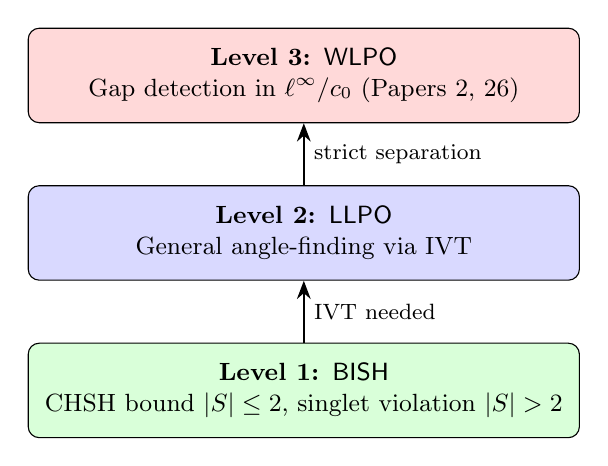
\begin{tikzpicture}[
  level/.style={draw, rounded corners, minimum width=7cm,
    minimum height=1.2cm, align=center, font=\small},
  >=Stealth
]
  \node[level, fill=green!15] (bish) at (0,0)
    {\textbf{Level 1: $\BISH$}\\
     CHSH bound $|S| \le 2$, singlet violation $|S| > 2$};
  \node[level, fill=blue!15] (llpo) at (0,2)
    {\textbf{Level 2: $\LLPO$}\\
     General angle-finding via IVT};
  \node[level, fill=red!15] (wlpo) at (0,4)
    {\textbf{Level 3: $\WLPO$}\\
     Gap detection in $\ell^\infty/c_0$ (Papers~2, 26)};
  \draw[->, thick] (bish) -- (llpo) node[midway, right, font=\footnotesize]
    {IVT needed};
  \draw[->, thick] (llpo) -- (wlpo) node[midway, right, font=\footnotesize]
    {strict separation};
\end{tikzpicture}
\caption{Three-level stratification of Bell-related computations in the
constructive hierarchy.  Each level adds decision capability strictly
beyond the previous one.}
\label{fig:stratification}
\end{figure}

\subsection{Comparison with Paper~26}

\begin{center}
\begin{tabular}{lll}
\toprule
\textbf{Feature} & \textbf{Paper~26} & \textbf{Paper~27} \\
\midrule
Principle & $\WLPO$ & $\LLPO$ \\
Physical space & $\ell^\infty/c_0$ & Bell correlations \\
Logical algebra & $\Pi^0_1/{\sim_{\mathsf{PA}}}$ & --- \\
Direction & Reduction (both directions) & Forward calibration \\
Detection & Zero $\Leftrightarrow$ refutable & Threshold crossing \\
Axioms & 5 & 6 \\
Sorries & 0 & 0 \\
\bottomrule
\end{tabular}
\end{center}

Together, Papers~26 and~27 provide two data points for the general
question: at what constructive strength does a given physical theory
require its key computations?  Gap detection needs~$\WLPO$;
angle-finding needs~$\LLPO$.  Whether calibrations at different levels
of the hierarchy share enough structural uniformity to support a
categorical framework remains open.  Papers~26 and~27 operate at
different constructive levels with different proof architectures
(reduction vs.\ forward calibration), so the evidence for uniform
structure is currently limited.

% ====================================================================
\section{Conclusion}\label{sec:conclusion}
% ====================================================================

We have formalized in Lean~4 the connection between $\LLPO$, the
Intermediate Value Theorem, and Bell angle optimization.  The main
result is a three-level stratification: specific violations are
$\BISH$-computable, general angle-finding requires exactly~$\LLPO$
(via IVT), and this is strictly below the~$\WLPO$ needed for gap
detection.

The formalization compiles cleanly (zero \texttt{sorry}, six cited
axioms) and explains the mechanism behind Paper~21's
$\LLPO \leftrightarrow \mathsf{BellSignDecision}$ equivalence: the IVT
is the mathematical content of~$\LLPO$, and root-finding is the
computational task underlying Bell angle optimization.

% ====================================================================
% References
% ====================================================================
\begin{thebibliography}{99}

\bibitem{BishopBridges1985}
E.~Bishop and D.~Bridges.
\newblock \emph{Constructive Analysis}.
\newblock Springer, 1985.

\bibitem{BridgesRichman1987}
D.~Bridges and F.~Richman.
\newblock \emph{Varieties of Constructive Mathematics}.
\newblock Cambridge University Press, 1987.

\bibitem{BridgesVita2006}
D.~Bridges and L.~V\^{\i}\c{t}\u{a}.
\newblock \emph{Techniques of Constructive Analysis}.
\newblock Springer, 2006.

\bibitem{Ishihara1989}
H.~Ishihara.
\newblock Continuity and nondiscontinuity in constructive mathematics.
\newblock \emph{J.~Symbolic Logic}, 56(4):1349--1354, 1991.

\bibitem{Ishihara2006}
H.~Ishihara.
\newblock Reverse mathematics in {B}ishop's constructive mathematics.
\newblock \emph{Philosophia Scientiae}, CS~6:43--59, 2006.

\bibitem{P21}
Foundation--Relativity Project.
\newblock Paper~21: {LLPO} and {B}ell sign decision---a {L}ean~4
  formalization.

\bibitem{P26}
Foundation--Relativity Project.
\newblock Paper~26: An arithmetic proof that bidual gap detection is
  {WLPO}-complete---a {L}ean~4 formalization.

\end{thebibliography}

\end{document}
